\section{Small Cap}
\begin{figure}[H]
\centering
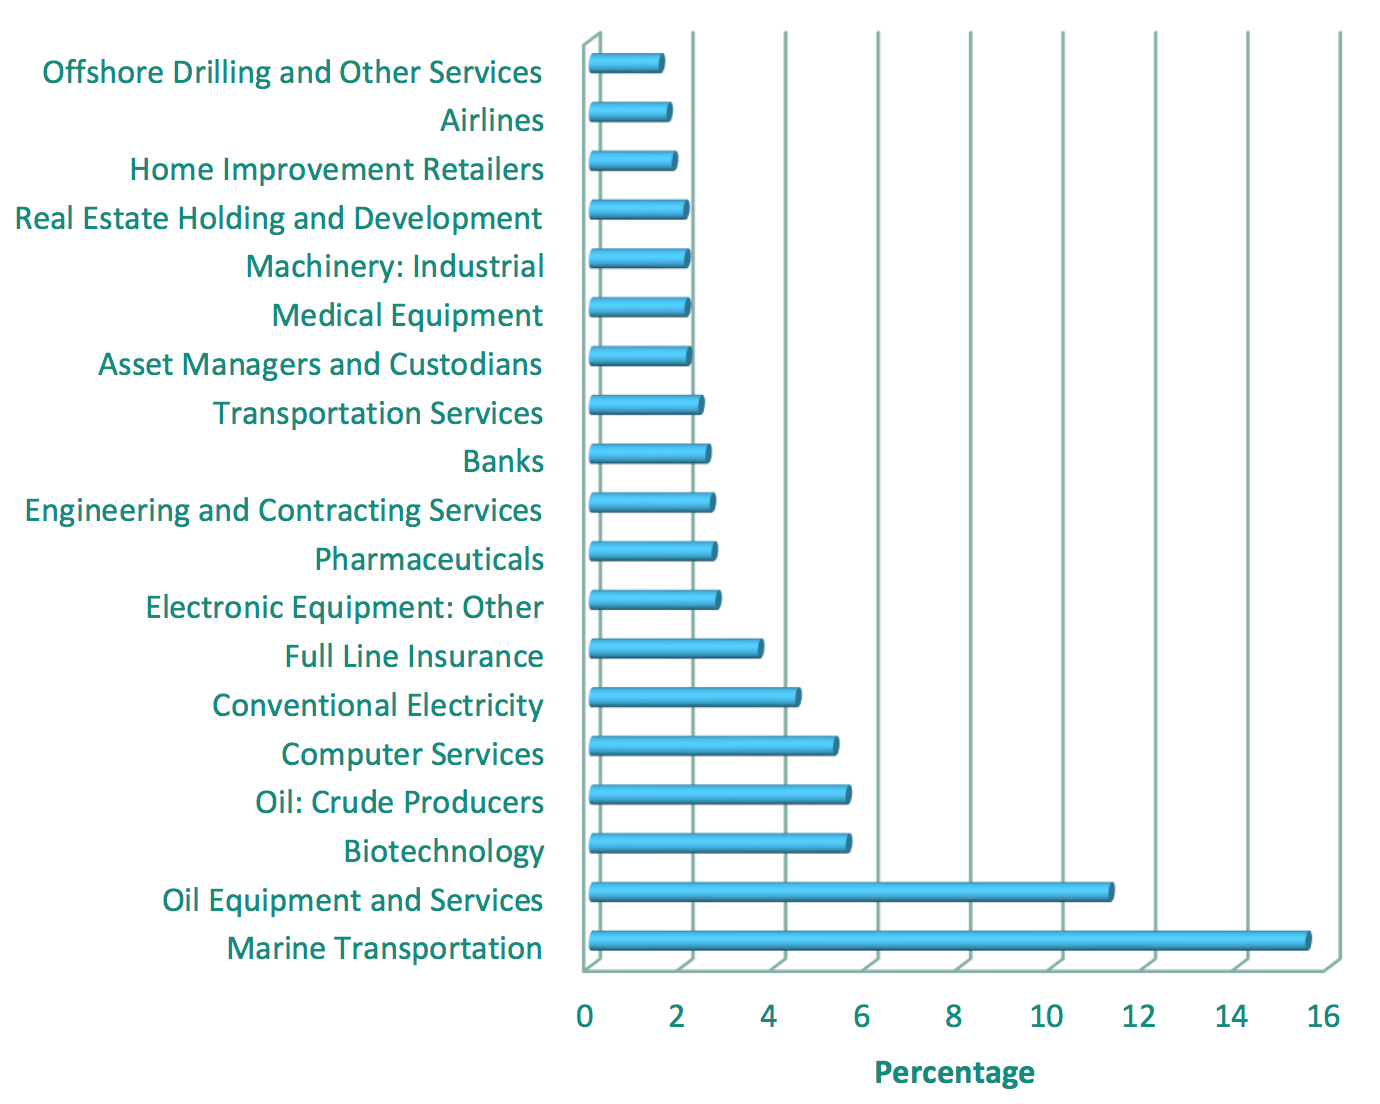
\includegraphics [scale=0.44,angle=360]{figures/smallsector.png}
\caption{OSESX Sector Allocation \cite{euronext}}
\label{fig:smallsector}
\end{figure}
\indent\newline 
Figure 3.1 shows the sector allocation of the small cap index as of 2021. The Index is dominated by marine transportation- and oil equipment and services companies, which accounts for approximately 25\% of the total index market cap. The smallest sectors consist of offshore drilling and airlines, and accounts for less than 2\% respectively of the total market cap. 

\indent\newline 
\begin{table}[ht]
\centering
\resizebox{\textwidth}{!}{\begin{tabular}{l|l}
\toprule
\textbf{Small cap statistics 2012-2020} \\ \midrule
Total number of stocks & 114 \\
Highest market capitalization & DOF Subsea (NOK 2,998,386,000 - 2012) \\
Lowest market capitalization & SeaBird Exploration (NOK 16,087,000 - 2017) \\
OSESX annualized returns  & 8.2\% \\ \bottomrule
\end{tabular}}
\caption{Small cap summary statistics}
\end{table}

\section{Large Cap}
\begin{figure}[H]
\centering
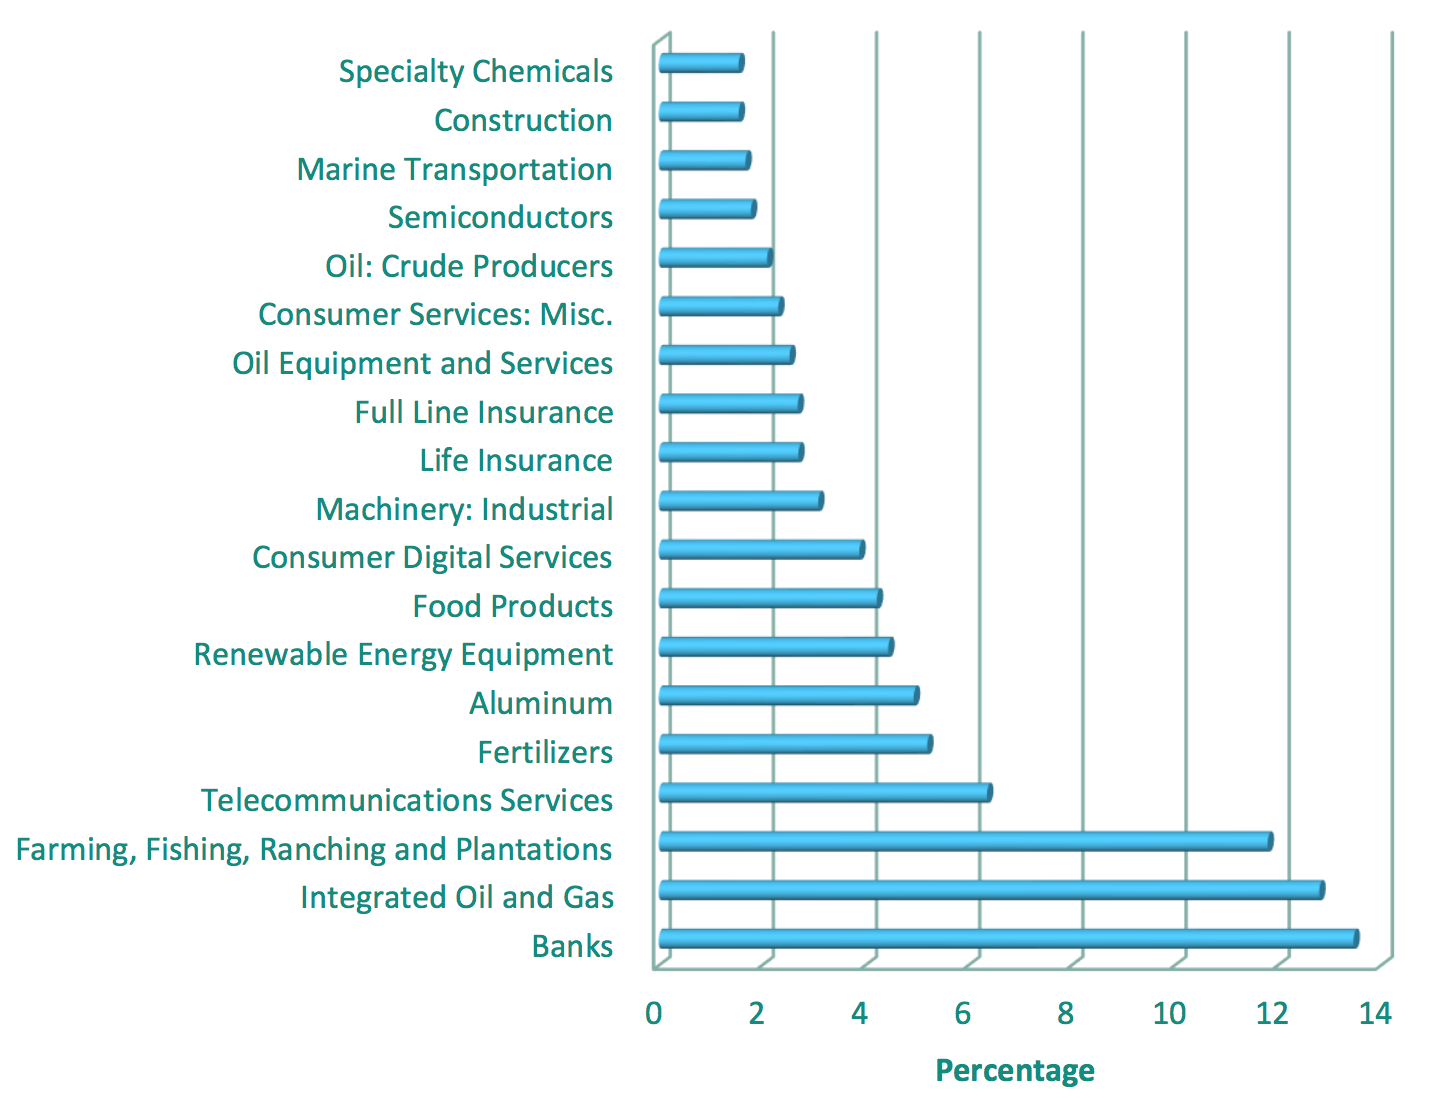
\includegraphics [scale=0.44,angle=360]{figures/largesector.png}
\caption{OSEBX Sector Allocation \cite{bors}}
\label{fig:largesector}
\end{figure}
\indent\newline 
Figure 3.2 illustrates the current sector allocation of the OSEBX index, mainly consisting of large cap stocks. The top three sectors are banks, integrated oil and gas, and farming, fishing, ranching and plantations, which represent approximately 38\% of the index total market cap. The bottom three sectors are specialty chemicals, construction, and marine transportation, where each sector makes up less than 2\% of the index. 

\indent\newline 
\begin{table}[ht]
\centering
\resizebox{\textwidth}{!}{\begin{tabular}{l|l}
\toprule
\textbf{Large cap statistics 2012-2020}  \\ \midrule
Total number of stocks & 64 \\
Highest market capitalization & Equinor (NOK 613,478,999,000 - 2018)  \\
Lowest market capitalization & Fjordkraft Holding (NOK 6,060,781,000 - 2019) \\
OSEBX annualized returns  & 16.7\% \\ \bottomrule
\end{tabular}}
\caption{Large cap summary statistics}
\end{table} 
